\documentclass{article}

\usepackage{url} 
\usepackage{geometry,afterpage}
\usepackage{pdfpages}
\usepackage{lastpage}
\usepackage{fancyhdr}
\usepackage{ngerman}
\usepackage{listings}

\usepackage{floatrow}
\usepackage[tableposition=top]{caption}
\floatsetup[table]{capposition=top}

\usepackage{amsmath, amssymb}

\usepackage[utf8]{inputenc}


\usepackage[numbib]{tocbibind}



\newcommand\twodigits[1]{%
   \ifnum#1<10 0#1\else #1\fi
}



\lhead{Röntgenbeugung}
\rhead{\today \\ J. Winkler}
%\cfoot{\twodigits{\thepage}~/ \pageref{LastPage}}
\cfoot{{\thepage}~/ \pageref{LastPage}}

\begin{document}

\parindent0cm


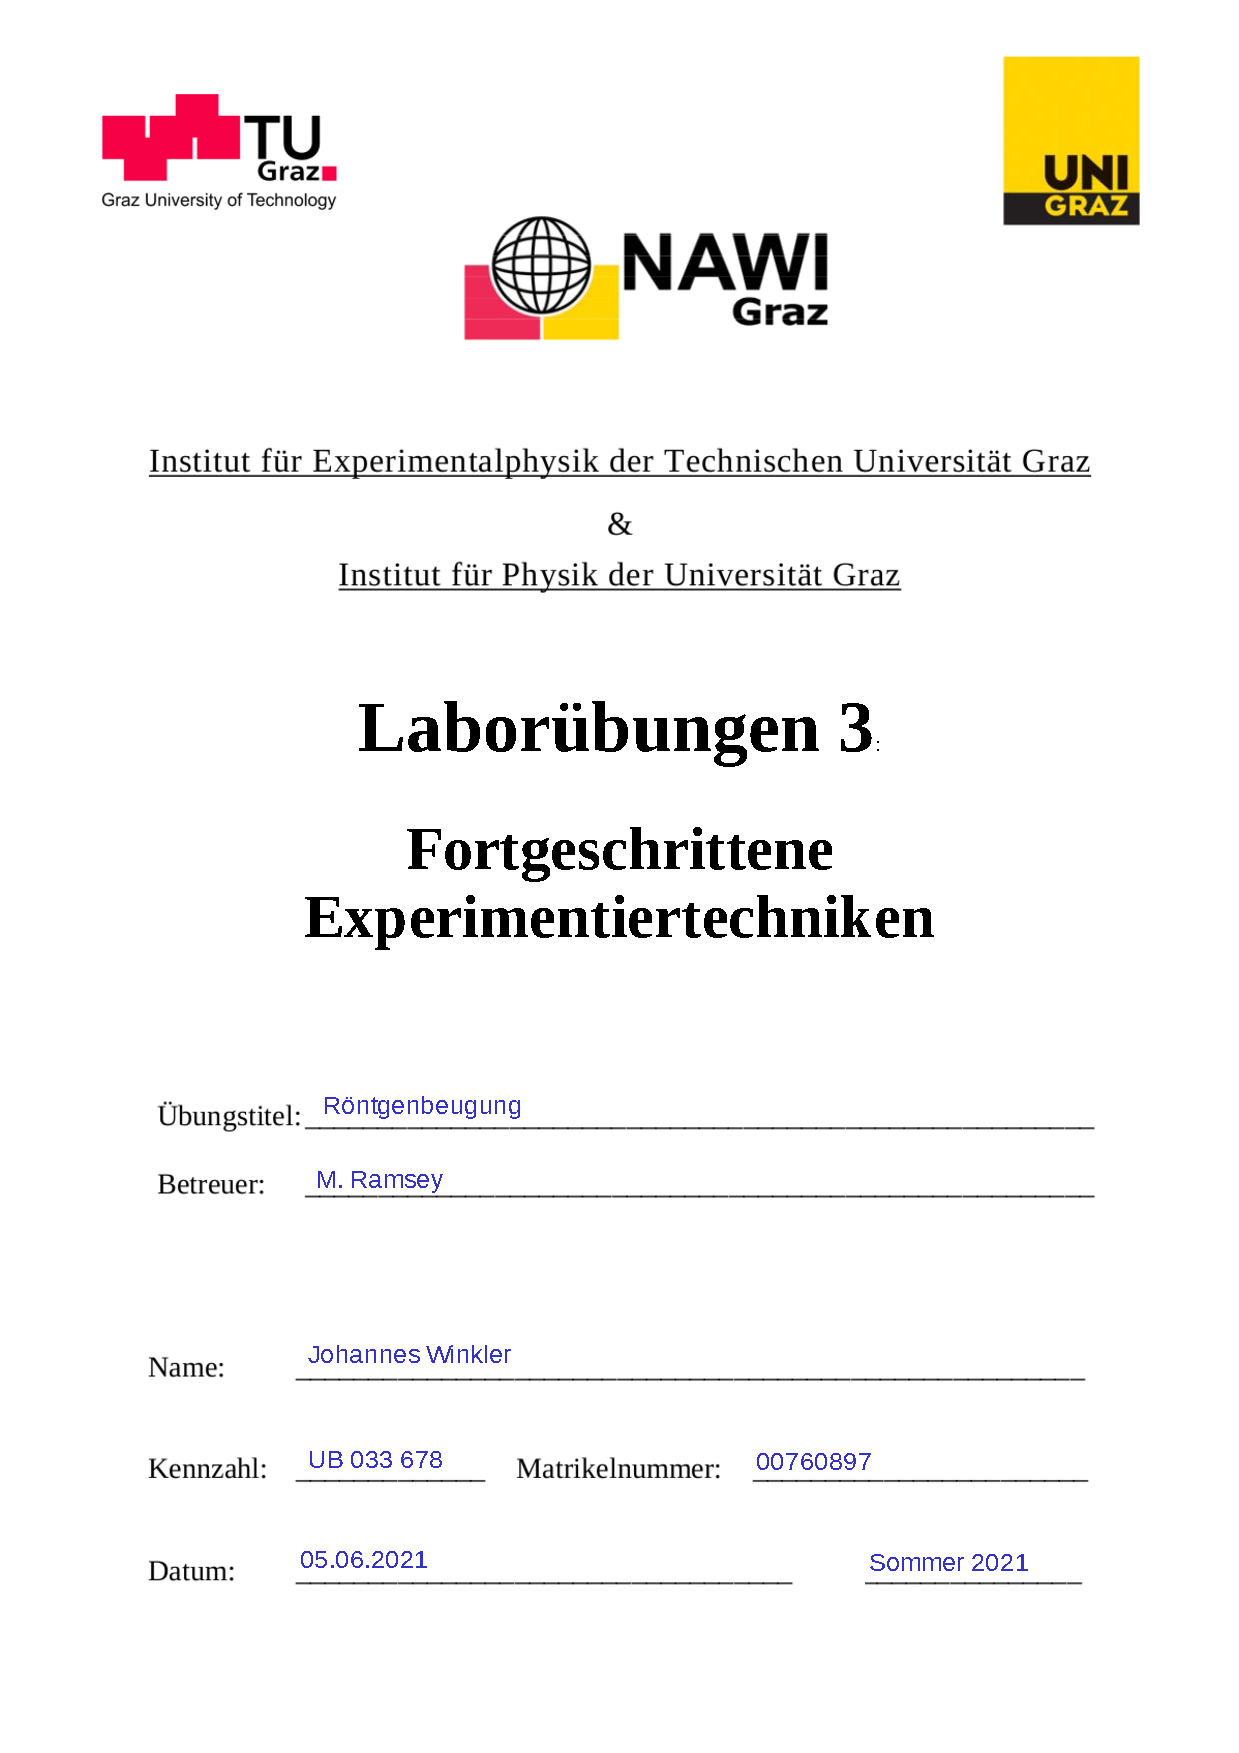
\includepdf{Deckblatt_neu_custom.pdf}


\pagestyle{fancy}

\section{Aufgabenstellung}

Die für das Experiment nötigen Daten inklusive der Aufgabenstellung wurden zur Verfügung gestellt. 

\begin{enumerate}
\item Bestimmung der Gitterkonstante von NaCl
\item Bestimmung der Gitterkonstante eines unbekannten Kristalls
\item Identifiation des unbekannten Kristalls
\item Berechnung der Grenzwellenlänge $\lambda_{\min}$ des Bremsstrahlungskontinuums in Abhängigkeit von der Spannung
\item Berechnung des Planck'schen Wirkungsquantums 
\end{enumerate}


\section{Grundlagen}

Röntgenstrahlung wird zur Bestimmung der Struktur fester Körper verwendet. Diese Strahlung besteht aus elektromagnetischen Wellen mit der Wellenlänge $10^{-12}$~m bis $10^{-10}$~m. Röntgenstrahlung entsteht beim Abbremsen von Elektronen und wird daher auch Bremsstrahlung genannt. Die schematische Darstellung einer Röntgenröhre befindet sich in Abbildung~\ref{fig:roentgenroehre}.



\begin{figure}[H]
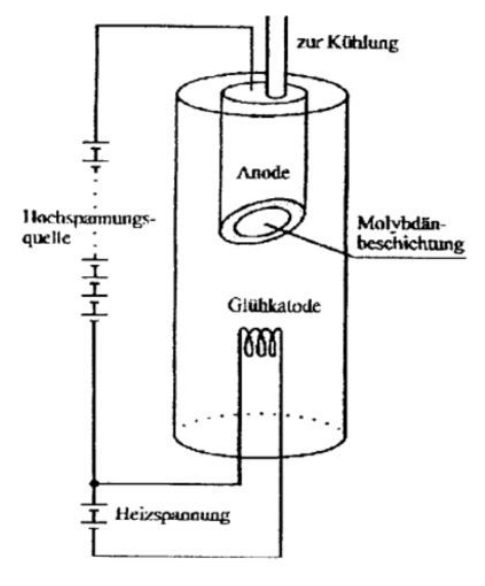
\includegraphics[scale=1.8]{roehre.png}
\caption{Der schematische Aufbau einer Röntgenröhre. In der Glühkathode werden Elektronen beschleunigt. Diese werden an der Anode abgebremst. Dadurch entsteht Röntgenstrahlung.}
\label{fig:roentgenroehre}
\end{figure}



\begin{figure}[H]
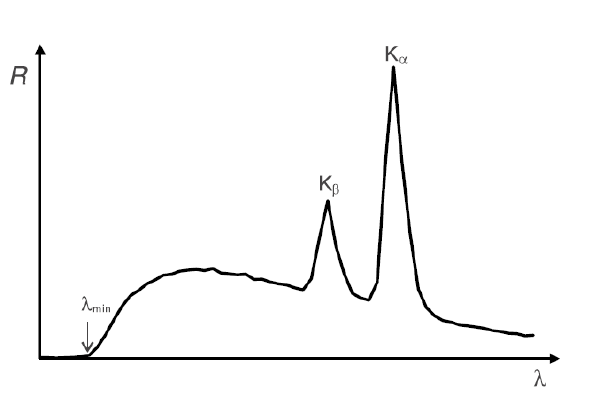
\includegraphics[scale=1.8]{alpha_beta.png}
\caption{Das Röntgenspektrum.}
\label{fig:roentgenspektrum}
\end{figure}

Das Spektrum der Bremsstrahlung ist kontinuierlich. Allerdings werden zusätzlich durch das Auftreffen der Elektronen die Atome der Anode ionisiert. Durch die Ionisation werden in der Atomhüller Löcher frei. Dadurch werden Energieniveaus der Elektronen verändert und die Energiedifferenz der Niveaus wird abgestrahlt. Das daraus entstehende so genannte \textit{Linienspektrum} besitzt zwei Maxima $K_\alpha$ und $K_\beta$, abhängig von den betroffenen Energieniveaus der ionisierten Elektronen. Es ist zu beobachten, dass $K_\beta$ eine höhere Energie aufweisen als $K_\alpha$ (daher kleinere Wellenlänge), aber dafür eine geringere Intensität, weil die $K_\alpha$-Ionisation häufiger vorkommt. Das Linienspektrum wird mit dem Bremsstrahlenspektrum überlagert und ist für jedes Material charakteristisch.


In Abbildung~\ref{fig:roentgenspektrum} sieht man zusätzlich noch $\lambda_{\min}$ eingezeichnet. Hierbei handelt es sich um die Grenzwellenlänge, also die minimale Wellenlänge von Röntgenstrahlung.



\begin{figure}[H]
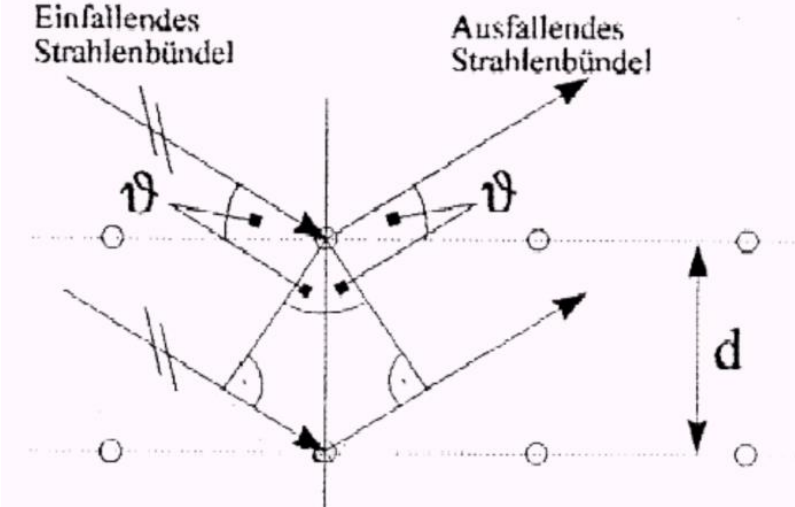
\includegraphics[scale=1.5]{bragg.png}
\caption{Veranschaulichung der Bragg-Bedingung.}
\label{fig:bragg}
\end{figure}


Für die Bestimmung der Gitterkonstante $a=2\cdot d$ wird gemäß \cite{moodle} die Bragg-Bedingung (siehe Abbildung~\ref{fig:bragg}) verwendet
\begin{align}
\label{eq:bragg}
n\cdot \lambda = 2\cdot d \cdot \sin(\vartheta)
\end{align}
verwendet, wobei $\lambda$ die Wellenlänge der $K_{\alpha}$ bzw. $K_{\beta}$ Strahlung in \cite{moodle} gegeben ist.
\begin{align}
\lambda(K_\alpha) &= (71.080 \pm 0.001)~\text{pm} \\
\lambda(K_\beta) &= (63.095 \pm 0.001)~\text{pm} 
\end{align}

Zusätzlich ist noch bekannt, dass es zwischen der Spannung und der Grenzwellenlänge folgenden Zusammenhang gibt
\begin{align}
\lambda_{\min} = \frac{h\cdot c}{e\cdot U}\label{eq:planck_formel}
\end{align}
wobei $c$ die Vakuumlichtgeschwindigkeit und $e$ die Elementarladung ist. Wenn $\lambda_{\min}$ und $U$ bekannt sind, kann damit das Planck'sche Wirkungsquantum näherungsweise bestimmt werden.




\section{Versuchsaufbau}


\begin{figure}[H]
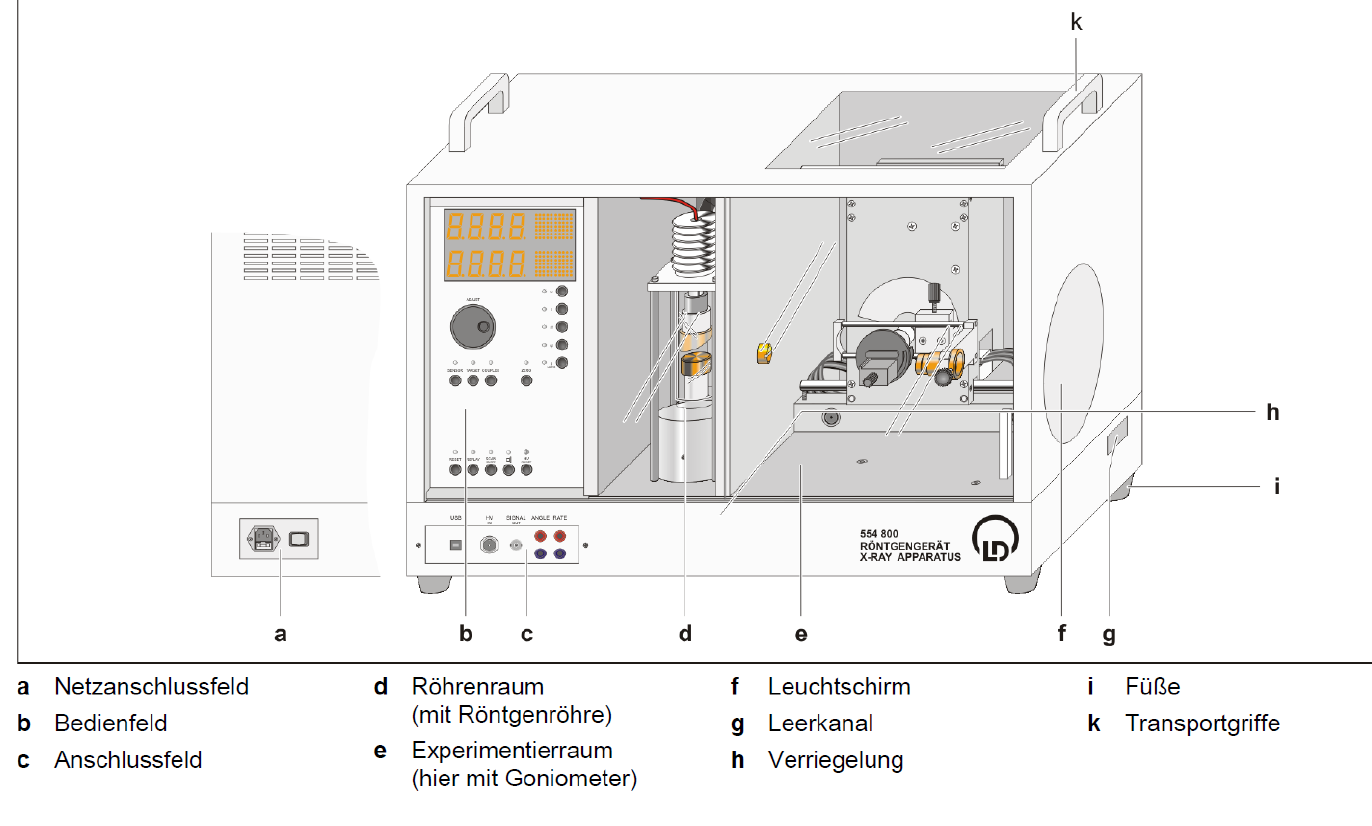
\includegraphics[scale=1]{aufbau.png}
\caption{Das Röntgengerät als Versuchsaufbau inkl. Beschreibung der Komponenten.}
\end{figure}


\begin{figure}[H]
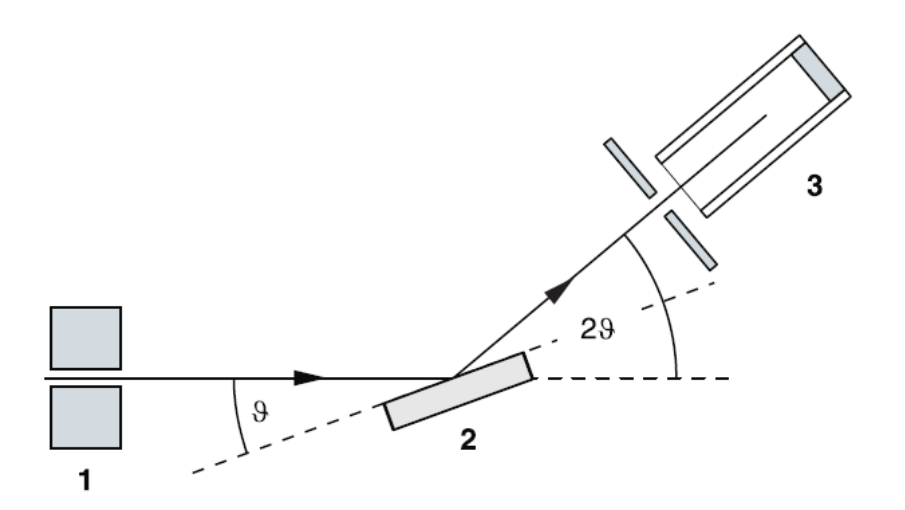
\includegraphics[scale=1]{versuch1.png}
\caption{Versuchsaufbau, dabei ist der \textbf{Kollimator} mit 1 markiert, der zu überprüfende \textbf{Kristall} mit 2 und an der Stelle 3 ist das \textbf{Zählrohr}.}
\end{figure}


\section{Geräteliste}


\begin{table}[H]
\caption{Liste der verwendeten Geräte}

~

\begin{tabular}{l|l}
Bezeichnung & Inventarnummer  \\
\hline
Röntgengerät & 554 811  \\
NaCl-Kristall &   \\
Kristall aus unbekannten Material & \\
Computer & \\
Geiger-Müller-Zählrohr & \\
CASSY-Lab Interface 
\end{tabular}

\end{table}


\section{Durchführung und Messergebnisse}

\subsection{Analyse von Kristallen}
Die Ergebnisse wurden gemessen und als Datensatz zur Verfügung gestellt. Der Vollständigkeit halber werden die Daten nochmals tabellarisch dargestellt. In Tabelle~\ref{tab:nacl} werden die Messergebnisse vom NaCl-Kristall zusammengefasst. Die Daten des unbekannten Kristalls sind in Tabelle~\ref{tab:kristall}.

Zum besseren Vergleich der Daten wurden diese in Abbildung~\ref{fig:daten} in ein gemeinsames Koordinatensystem eingezeichnet.

\begin{figure}[H]
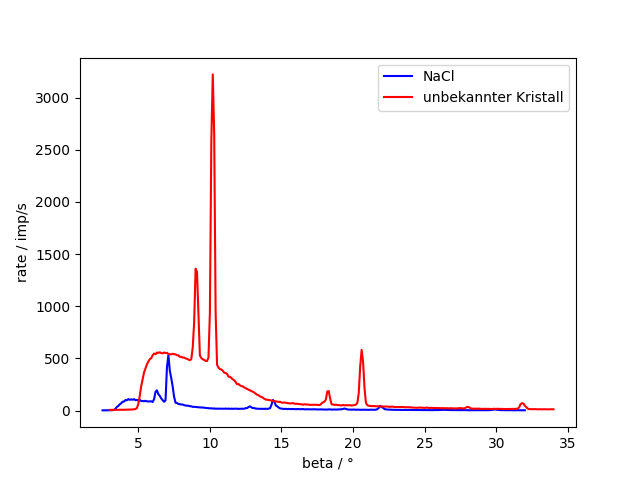
\includegraphics[scale=1]{daten.png}
\caption{Daten der beiden Kristalle}
\label{fig:daten}
\end{figure}


\newpage
\begin{table}[H]
\caption{Begungsdaten für NaCl. $\beta$ in $^\circ$, rate in imp/s.}
\small
\begin{tabular}{rr|rr|rr|rr|rr|rr}
$\beta$ & rate & $\beta$ & rate & $\beta$ & rate & $\beta$ & rate & $\beta$ & rate & $\beta$ & rate \\
\hline
2.5	&	2.50	&	7.4	&	230.83	&	12.3	&	18.20	&	17.2	&	12.60	&	22.1	&	25.67	&	27.0	&	4.77\\
2.6	&	2.50	&	7.5	&	131.10	&	12.4	&	17.77	&	17.3	&	12.60	&	22.2	&	14.43	&	27.1	&	4.30\\
2.7	&	1.77	&	7.6	&	74.73	&	12.5	&	23.33	&	17.4	&	11.50	&	22.3	&	11.90	&	27.2	&	4.50\\
2.8	&	1.83	&	7.7	&	72.50	&	12.6	&	24.07	&	17.5	&	11.67	&	22.4	&	9.80	&	27.3	&	4.47\\
2.9	&	2.40	&	7.8	&	63.37	&	12.7	&	34.17	&	17.6	&	10.17	&	22.5	&	9.20	&	27.4	&	4.70\\
3.0	&	2.83	&	7.9	&	60.50	&	12.8	&	40.60	&	17.7	&	11.83	&	22.6	&	7.97	&	27.5	&	4.37\\
3.1	&	3.13	&	8.0	&	58.57	&	12.9	&	30.10	&	17.8	&	10.70	&	22.7	&	7.03	&	27.6	&	4.30\\
3.2	&	4.20	&	8.1	&	58.07	&	13.0	&	24.20	&	17.9	&	10.43	&	22.8	&	7.77	&	27.7	&	4.43\\
3.3	&	6.50	&	8.2	&	51.60	&	13.1	&	23.83	&	18.0	&	10.27	&	22.9	&	6.40	&	27.8	&	4.00\\
3.4	&	16.93	&	8.3	&	48.60	&	13.2	&	19.50	&	18.1	&	9.73	&	23.0	&	6.83	&	27.9	&	4.03\\
3.5	&	34.67	&	8.4	&	47.17	&	13.3	&	18.17	&	18.2	&	9.63	&	23.1	&	6.73	&	28.0	&	4.07\\
3.6	&	44.20	&	8.5	&	46.33	&	13.4	&	17.30	&	18.3	&	11.90	&	23.2	&	6.40	&	28.1	&	3.20\\
3.7	&	60.20	&	8.6	&	41.47	&	13.5	&	16.73	&	18.4	&	10.43	&	23.3	&	6.87	&	28.2	&	3.33\\
3.8	&	69.20	&	8.7	&	40.80	&	13.6	&	16.63	&	18.5	&	9.93	&	23.4	&	7.47	&	28.3	&	3.63\\
3.9	&	85.17	&	8.8	&	35.83	&	13.7	&	17.03	&	18.6	&	9.37	&	23.5	&	6.83	&	28.4	&	4.07\\
4.0	&	86.03	&	8.9	&	36.17	&	13.8	&	15.80	&	18.7	&	10.90	&	23.6	&	5.63	&	28.5	&	4.13\\
4.1	&	101.23	&	9.0	&	34.77	&	13.9	&	18.57	&	18.8	&	9.60	&	23.7	&	6.67	&	28.6	&	4.17\\
4.2	&	98.53	&	9.1	&	34.40	&	14.0	&	15.70	&	18.9	&	10.13	&	23.8	&	6.63	&	28.7	&	3.90\\
4.3	&	109.80	&	9.2	&	31.23	&	14.1	&	18.43	&	19.0	&	11.23	&	23.9	&	5.80	&	28.8	&	3.77\\
4.4	&	102.90	&	9.3	&	30.33	&	14.2	&	22.10	&	19.1	&	11.03	&	24.0	&	5.27	&	28.9	&	4.53\\
4.5	&	107.80	&	9.4	&	29.13	&	14.3	&	54.90	&	19.2	&	12.70	&	24.1	&	5.90	&	29.0	&	3.13\\
4.6	&	103.33	&	9.5	&	30.00	&	14.4	&	101.53	&	19.3	&	15.93	&	24.2	&	6.63	&	29.1	&	3.57\\
4.7	&	109.90	&	9.6	&	27.27	&	14.5	&	87.87	&	19.4	&	19.37	&	24.3	&	5.67	&	29.2	&	3.87\\
4.8	&	99.47	&	9.7	&	26.07	&	14.6	&	50.53	&	19.5	&	16.33	&	24.4	&	6.17	&	29.3	&	4.03\\
4.9	&	102.23	&	9.8	&	23.80	&	14.7	&	41.30	&	19.6	&	11.33	&	24.5	&	5.50	&	29.4	&	3.93\\
5.0	&	96.17	&	9.9	&	23.07	&	14.8	&	29.97	&	19.7	&	10.27	&	24.6	&	5.80	&	29.5	&	3.73\\
5.1	&	101.93	&	10.0	&	20.97	&	14.9	&	20.53	&	19.8	&	8.93	&	24.7	&	5.67	&	29.6	&	4.90\\
5.2	&	91.53	&	10.1	&	22.03	&	15.0	&	18.30	&	19.9	&	9.43	&	24.8	&	5.37	&	29.7	&	5.20\\
5.3	&	91.80	&	10.2	&	19.47	&	15.1	&	17.10	&	20.0	&	9.33	&	24.9	&	5.83	&	29.8	&	8.20\\
5.4	&	89.13	&	10.3	&	20.70	&	15.2	&	14.93	&	20.1	&	9.80	&	25.0	&	5.43	&	29.9	&	11.10\\
5.5	&	93.87	&	10.4	&	17.23	&	15.3	&	17.13	&	20.2	&	7.80	&	25.1	&	5.17	&	30.0	&	8.18\\
5.6	&	87.93	&	10.5	&	18.63	&	15.4	&	14.17	&	20.3	&	8.80	&	25.2	&	5.13	&	30.1	&	6.93\\
5.7	&	88.57	&	10.6	&	18.50	&	15.5	&	16.27	&	20.4	&	7.83	&	25.3	&	4.43	&	30.2	&	6.33\\
5.8	&	87.37	&	10.7	&	19.17	&	15.6	&	14.57	&	20.5	&	7.90	&	25.4	&	4.47	&	30.3	&	4.53\\
5.9	&	89.63	&	10.8	&	17.43	&	15.7	&	15.03	&	20.6	&	7.33	&	25.5	&	4.93	&	30.4	&	3.77\\
6.0	&	82.40	&	10.9	&	18.87	&	15.8	&	15.03	&	20.7	&	8.63	&	25.6	&	4.20	&	30.5	&	4.90\\
6.1	&	108.33	&	11.0	&	17.70	&	15.9	&	14.07	&	20.8	&	8.20	&	25.7	&	6.03	&	30.6	&	3.83\\
6.2	&	179.63	&	11.1	&	19.00	&	16.0	&	13.70	&	20.9	&	8.43	&	25.8	&	5.00	&	30.7	&	4.33\\
6.3	&	194.53	&	11.2	&	17.33	&	16.1	&	14.73	&	21.0	&	7.97	&	25.9	&	5.07	&	30.8	&	3.93\\
6.4	&	156.70	&	11.3	&	18.97	&	16.2	&	14.30	&	21.1	&	7.27	&	26.0	&	4.70	&	30.9	&	3.07\\
6.5	&	141.03	&	11.4	&	16.50	&	16.3	&	13.93	&	21.2	&	8.50	&	26.1	&	5.33	&	31.0	&	4.33\\
6.6	&	116.30	&	11.5	&	18.67	&	16.4	&	13.20	&	21.3	&	7.93	&	26.2	&	5.90	&	31.1	&	3.53\\
6.7	&	100.80	&	11.6	&	16.87	&	16.5	&	15.20	&	21.4	&	8.03	&	26.3	&	7.23	&	31.2	&	2.60\\
6.8	&	84.17	&	11.7	&	17.90	&	16.6	&	11.50	&	21.5	&	7.73	&	26.4	&	8.07	&	31.3	&	3.47\\
6.9	&	97.67	&	11.8	&	18.57	&	16.7	&	12.83	&	21.6	&	8.53	&	26.5	&	6.07	&	31.4	&	3.43\\
7.0	&	416.53	&	11.9	&	17.30	&	16.8	&	12.13	&	21.7	&	13.93	&	26.6	&	5.53	&	31.5	&	3.10\\
7.1	&	532.37	&	12.0	&	16.40	&	16.9	&	12.63	&	21.8	&	26.00	&	26.7	&	4.03	&	31.6	&	2.97\\
7.2	&	381.63	&	12.1	&	17.33	&	17.0	&	11.73	&	21.9	&	45.67	&	26.8	&	4.73	&	31.7	&	3.40\\
7.3	&	310.73	&	12.2	&	18.13	&	17.1	&	12.00	&	22.0	&	33.50	&	26.9	&	4.73	&	31.8	&	2.90\\

\end{tabular}
\label{tab:nacl}
\end{table}

\newpage

\begin{table}[H]
\caption{Begungsdaten für den unbekannten Kristall. $\beta$ in $^\circ$, rate in imp/s.}
\small
\begin{tabular}{rr|rr|rr|rr|rr|rr|rr}
$\beta$ & rate & $\beta$ & rate & $\beta$ & rate & $\beta$ & rate & $\beta$ & rate & $\beta$ & rate & $\beta$ & rate \\
\hline
3.0	&	6.57	&	7.9	&	514.87	&	12.8	&	193.57	&	17.7	&	54.17	&	22.6	&	36.37	&	27.5	&	24.37	&	32.4	&	13.47\\
3.1	&	6.53	&	8.0	&	515.87	&	12.9	&	187.10	&	17.8	&	68.43	&	22.7	&	38.17	&	27.6	&	21.67	&	32.5	&	14.00\\
3.2	&	6.20	&	8.1	&	508.10	&	13.0	&	180.10	&	17.9	&	79.07	&	22.8	&	36.87	&	27.7	&	21.13	&	32.6	&	13.03\\
3.3	&	7.17	&	8.2	&	508.17	&	13.1	&	173.20	&	18.0	&	85.27	&	22.9	&	34.27	&	27.8	&	22.10	&	32.7	&	14.30\\
3.4	&	7.30	&	8.3	&	500.00	&	13.2	&	161.30	&	18.1	&	104.93	&	23.0	&	33.70	&	27.9	&	30.37	&	32.8	&	12.57\\
3.5	&	6.10	&	8.4	&	495.77	&	13.3	&	152.40	&	18.2	&	183.40	&	23.1	&	34.23	&	28.0	&	35.47	&	32.9	&	12.47\\
3.6	&	7.07	&	8.5	&	489.70	&	13.4	&	146.67	&	18.3	&	186.90	&	23.2	&	33.87	&	28.1	&	32.27	&	33.0	&	12.80\\
3.7	&	8.17	&	8.6	&	482.47	&	13.5	&	136.47	&	18.4	&	115.90	&	23.3	&	33.37	&	28.2	&	22.07	&	33.1	&	13.43\\
3.8	&	7.47	&	8.7	&	493.13	&	13.6	&	130.77	&	18.5	&	60.57	&	23.4	&	35.00	&	28.3	&	20.37	&	33.2	&	11.27\\
3.9	&	7.40	&	8.8	&	605.20	&	13.7	&	123.67	&	18.6	&	58.80	&	23.5	&	33.27	&	28.4	&	17.70	&	33.3	&	13.00\\
4.0	&	7.87	&	8.9	&	846.43	&	13.8	&	113.43	&	18.7	&	53.67	&	23.6	&	32.30	&	28.5	&	18.60	&	33.4	&	12.57\\
4.1	&	8.23	&	9.0	&	1360.53	&	13.9	&	106.03	&	18.8	&	57.33	&	23.7	&	32.23	&	28.6	&	18.73	&	33.5	&	13.00\\
4.2	&	8.83	&	9.1	&	1326.77	&	14.0	&	104.13	&	18.9	&	53.00	&	23.8	&	31.23	&	28.7	&	17.77	&	33.6	&	12.23\\
4.3	&	9.50	&	9.2	&	933.97	&	14.1	&	102.10	&	19.0	&	52.73	&	23.9	&	32.00	&	28.8	&	19.23	&	33.7	&	11.70\\
4.4	&	10.17	&	9.3	&	528.57	&	14.2	&	99.07	&	19.1	&	50.47	&	24.0	&	30.33	&	28.9	&	16.63	&	33.8	&	12.83\\
4.5	&	11.23	&	9.4	&	502.97	&	14.3	&	95.27	&	19.2	&	49.80	&	24.1	&	29.47	&	29.0	&	16.33	&	33.9	&	12.50\\
4.6	&	10.73	&	9.5	&	491.63	&	14.4	&	93.87	&	19.3	&	53.60	&	24.2	&	29.20	&	29.1	&	16.27	&	34.0	&	12.30\\
4.7	&	12.33	&	9.6	&	486.10	&	14.5	&	87.83	&	19.4	&	50.20	&	24.3	&	28.17	&	29.2	&	16.97	&	\\
4.8	&	14.43	&	9.7	&	475.47	&	14.6	&	89.03	&	19.5	&	51.60	&	24.4	&	27.47	&	29.3	&	17.10	&	\\
4.9	&	23.77	&	9.8	&	474.60	&	14.7	&	86.23	&	19.6	&	51.83	&	24.5	&	26.70	&	29.4	&	15.10	&	\\
5.0	&	65.10	&	9.9	&	508.90	&	14.8	&	83.27	&	19.7	&	50.07	&	24.6	&	28.70	&	29.5	&	16.63	&	\\
5.1	&	141.10	&	10.0	&	937.87	&	14.9	&	84.63	&	19.8	&	52.13	&	24.7	&	28.37	&	29.6	&	16.17	&	\\
5.2	&	234.00	&	10.1	&	2591.13	&	15.0	&	77.23	&	19.9	&	47.77	&	24.8	&	28.17	&	29.7	&	14.93	&	\\
5.3	&	302.30	&	10.2	&	3222.53	&	15.1	&	75.07	&	20.0	&	50.40	&	24.9	&	26.60	&	29.8	&	16.80	&	\\
5.4	&	366.07	&	10.3	&	2650.13	&	15.2	&	77.60	&	20.1	&	52.07	&	25.0	&	25.90	&	29.9	&	16.07	&	\\
5.5	&	403.50	&	10.4	&	938.77	&	15.3	&	75.47	&	20.2	&	56.70	&	25.1	&	27.83	&	30.0	&	16.10	&	\\
5.6	&	443.10	&	10.5	&	439.33	&	15.4	&	72.03	&	20.3	&	73.50	&	25.2	&	28.40	&	30.1	&	17.17	&	\\
5.7	&	469.27	&	10.6	&	411.43	&	15.5	&	70.40	&	20.4	&	171.23	&	25.3	&	24.87	&	30.2	&	16.50	&	\\
5.8	&	493.03	&	10.7	&	397.37	&	15.6	&	68.57	&	20.5	&	425.73	&	25.4	&	26.20	&	30.3	&	15.90	&	\\
5.9	&	503.33	&	10.8	&	394.80	&	15.7	&	69.10	&	20.6	&	581.33	&	25.5	&	25.70	&	30.4	&	16.23	&	\\
6.0	&	529.60	&	10.9	&	380.67	&	15.8	&	71.10	&	20.7	&	467.13	&	25.6	&	24.93	&	30.5	&	14.57	&	\\
6.1	&	546.77	&	11.0	&	363.83	&	15.9	&	66.70	&	20.8	&	216.80	&	25.7	&	24.93	&	30.6	&	15.40	&	\\
6.2	&	540.03	&	11.1	&	359.70	&	16.0	&	65.30	&	20.9	&	73.83	&	25.8	&	24.73	&	30.7	&	14.17	&	\\
6.3	&	556.13	&	11.2	&	351.27	&	16.1	&	65.70	&	21.0	&	51.30	&	25.9	&	24.17	&	30.8	&	15.57	&	\\
6.4	&	552.90	&	11.3	&	324.70	&	16.2	&	62.47	&	21.1	&	45.93	&	26.0	&	23.27	&	30.9	&	15.20	&	\\
6.5	&	558.93	&	11.4	&	323.67	&	16.3	&	61.10	&	21.2	&	44.73	&	26.1	&	23.20	&	31.0	&	15.03	&	\\
6.6	&	550.33	&	11.5	&	312.30	&	16.4	&	60.20	&	21.3	&	42.87	&	26.2	&	23.33	&	31.1	&	15.57	&	\\
6.7	&	549.40	&	11.6	&	299.20	&	16.5	&	56.47	&	21.4	&	42.33	&	26.3	&	23.90	&	31.2	&	16.53	&	\\
6.8	&	556.73	&	11.7	&	289.93	&	16.6	&	60.93	&	21.5	&	43.80	&	26.4	&	22.93	&	31.3	&	15.20	&	\\
6.9	&	551.57	&	11.8	&	272.70	&	16.7	&	58.67	&	21.6	&	40.57	&	26.5	&	21.53	&	31.4	&	16.97	&	\\
7.0	&	553.50	&	11.9	&	252.43	&	16.8	&	58.30	&	21.7	&	41.63	&	26.6	&	23.43	&	31.5	&	18.73	&	\\
7.1	&	542.83	&	12.0	&	254.70	&	16.9	&	57.30	&	21.8	&	40.63	&	26.7	&	20.83	&	31.6	&	30.70	&	\\
7.2	&	540.83	&	12.1	&	242.23	&	17.0	&	54.40	&	21.9	&	39.50	&	26.8	&	22.53	&	31.7	&	60.93	&	\\
7.3	&	538.67	&	12.2	&	234.27	&	17.1	&	54.93	&	22.0	&	38.67	&	26.9	&	22.57	&	31.8	&	70.87	&	\\
7.4	&	544.80	&	12.3	&	231.93	&	17.2	&	56.33	&	22.1	&	39.57	&	27.0	&	20.60	&	31.9	&	66.80	&	\\
7.5	&	540.03	&	12.4	&	221.90	&	17.3	&	55.00	&	22.2	&	38.50	&	27.1	&	21.17	&	32.0	&	47.50	&	\\
7.6	&	539.60	&	12.5	&	214.33	&	17.4	&	56.20	&	22.3	&	38.27	&	27.2	&	20.67	&	32.1	&	32.87	&	\\
7.7	&	530.30	&	12.6	&	207.17	&	17.5	&	54.93	&	22.4	&	39.20	&	27.3	&	21.27	&	32.2	&	18.93	&	\\
7.8	&	529.27	&	12.7	&	200.77	&	17.6	&	53.00	&	22.5	&	36.10	&	27.4	&	22.43	&	32.3	&	14.27	&	\\

\end{tabular}
\label{tab:kristall}
\end{table}

\subsection{Planck'sches Wirkungsquantum}


Zusätzlich war das Planck'sche Wirkungsquantum zu bestimmen. Dazu waren weitere Datenreihen gegeben, die in Grafik~\ref{fig:planck} visualisiert sind.

\begin{figure}[H]
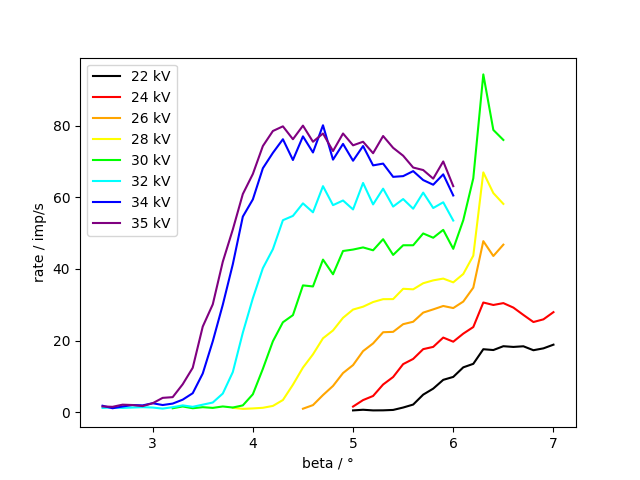
\includegraphics[scale=0.9]{planck.png}
\caption{Visualisierte Datenreihen des Planck'schen Wirkungsquantums}
\label{fig:planck}
\end{figure}




\section{Auswertung}
\subsection{Analyse von Kristallen}
Für beide Kristalle können die Maxima gefunden werden. Diese werden dann nach $K_\alpha$ und $K_\beta$ kategorisiert in den Tabellen~\ref{tab:auswertung_nacl} und~\ref{tab:auswertung_unkonwn} zusammengefasst.

\begin{figure}[H]
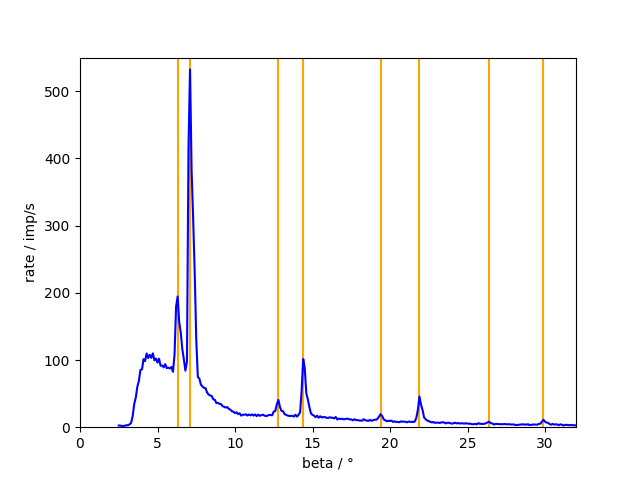
\includegraphics[scale=0.7]{daten_nacl.png}
\caption{Gemessene Röntgenbeugung am NaCl-Kristall mit orange markierten Maxima.}
\end{figure}



\begin{figure}[H]
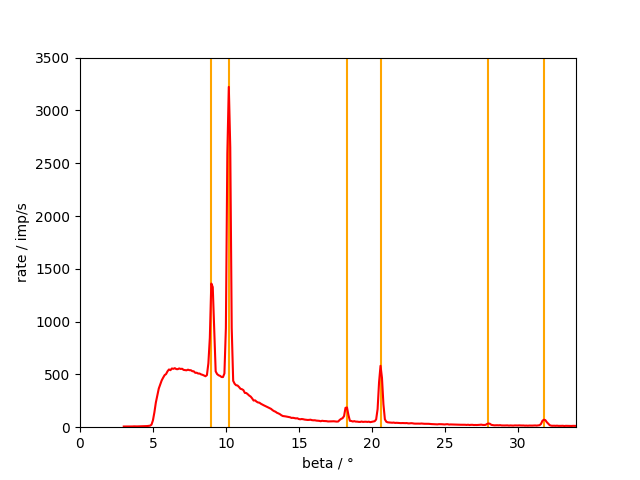
\includegraphics[scale=0.7]{daten_kristall.png}
\caption{Gemessene Röntgenbeugung am unbekannten Kristall mit orange markierten Maxima.}
\end{figure}


\begin{table}[H]
\centering
\caption{Auswertung der Peaks beim NaCl-Kristall.}
\label{tab:auswertung_nacl}
\begin{tabular}{rr|rr}
\multicolumn{2}{c|}{$K_\beta$} & \multicolumn{2}{c}{$K_\alpha$} \\ 
$\beta~/~^\circ$ & rate~/~ imp/s & $\beta~/~^\circ$ & rate~/~ imp/s \\
\hline
6.3 & 194.53 & 7.1 & 532.37 \\
12.8 & 40.60 & 14.4 & 101.53 \\
19.4 & 19.37 & 21.9 & 45.67 \\
26.4 & 8.07 & 29.9 & 11.10
\end{tabular}
\label{tab:peaks_nacl}
\end{table}


\begin{table}[H]
\centering
\caption{Auswertung der Peaks beim unbekannten Kristall.}\label{tab:auswertung_unkonwn}
\begin{tabular}{rr|rr}
\multicolumn{2}{c|}{$K_\beta$} & \multicolumn{2}{c}{$K_\alpha$} \\ 
$\beta~/~^\circ$ & rate~/~ imp/s & $\beta~/~^\circ$ & rate~/~ imp/s \\
\hline
9.0 & 1360.53 & 10.2 & 3222.50 \\
18.3 & 186.90 & 20.6 & 581.33 \\
28.0 & 35.47 & 31.8 & 70.87
\end{tabular}
\label{tab:peaks_kristall}
\end{table}




Nach Gleichung~\eqref{fig:bragg} und $a=2\cdot d$ kann die Gitterkonstante nun berechnet werden. Es gilt mit Fehlerrechnung
\begin{align}
a = \frac{n\cdot \lambda}{\sin(\vartheta)} \pm \left( \frac{n\cdot \Delta \lambda}{\sin(\vartheta)} + \frac{n\cdot \lambda}{\sin^2(\vartheta)}\cdot \cos(\vartheta) \cdot \Delta \theta\right)
\label{eq:gitterkonst_fehler} 
\end{align}



\begin{table}[H]
\centering
\caption{Berechnung der Gitterkonstante beim NaCl-Kristall.}
\label{tab:gitterkonst_nacl}
\begin{tabular}{rr|rr}
\multicolumn{2}{c|}{$K_\beta$} & \multicolumn{2}{c}{$K_\alpha$} \\ 
$a$ / pm & $\Delta a$ /pm & $a$ / pm & $\Delta a$ / pm\\
\hline
575.0 & 9.1 & 575.1 & 8.1 \\
569.6 & 4.4 & 571.6 & 3.9 \\
569.9 & 2.8 & 571.7 & 2.5 \\
567.6 & 2.0 & 570.4 & 1.7 
\end{tabular}
\end{table}



\begin{table}[H]
\centering
\caption{Berechnung der Gitterkonstante beim unbekannten Kristall.}
\label{tab:gitterkonst_unkonwn}
\begin{tabular}{rr|rr}
\multicolumn{2}{c|}{$K_\beta$} & \multicolumn{2}{c}{$K_\alpha$} \\ 
$a$ / pm & $\Delta a$ /pm & $a$ / pm & $\Delta a$ / pm\\
\hline
403.3 & 4.5 & 401.4 & 3.9 \\
401.9 & 2.1 & 404.0 & 1.9 \\
403.2 & 1.3 & 404.7 & 1.1
\end{tabular}
\end{table}

Als Gitterkonstante für den NaCl-Kristall ergibt sich
\begin{align*}
a_\text{NaCl} = (571.4\pm 9.1)~\text{pm}
\end{align*}

Als Gitterkonstante für den unbekannten Kristall ergibt sich
\begin{align*}
a_\text{LiF} = (403.1\pm 4.5)~\text{pm}
\end{align*}


\subsection{Planck'sches Wirkungsquantum}

Für die Bestimmung des Planck'schen Wirkungsquantums wurde über den linearen Teil der Kurven aus Grafik~\ref{fig:planck} eine Regressionsgerade bestimmt, um die Nullstelle zu finden. Das Ergebnis ist in Grafik~\ref{fig:planck_regression} visualisiert. Die Nullstellen finden sich in Tabelle~\ref{tab:planck_calc}. In dieser Tabelle sind zusätzlich die Grenzwellenlängen $\lambda_{\min}$ angegeben, welche mit Gleichung~\eqref{eq:bragg} berechnet wurden. Aus diesen kann letztendlich das Planck'sche Wirkungsquantum mit Formel~\eqref{eq:planck_formel} berechnet werden.


\begin{figure}[H]
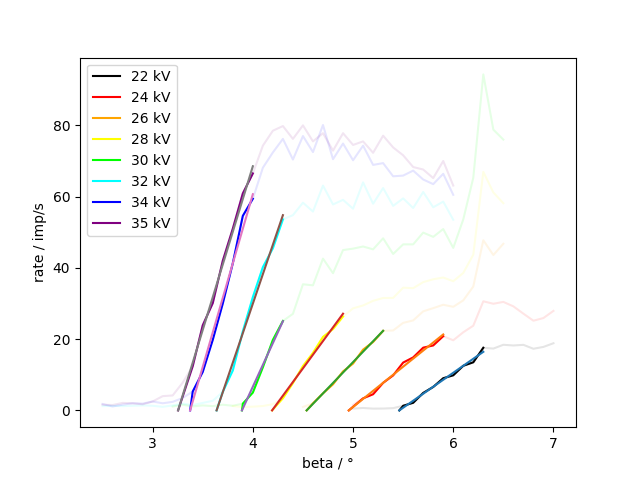
\includegraphics[scale=0.9]{planck_regression.png}
\caption{Visualisierte Datenreihen des Planck'schen Wirkungsquantums mit Regression zum Finden der Nullstelle.}
\label{fig:planck_regression}
\end{figure}


\begin{table}[H]
\caption{Nullstellen der Regressionsgeraden und Grenzwellenlängen $\lambda_{\min}$ (berechnet aus Gleichung~\ref{eq:bragg}) für die Bestimmung des Planck'schen Wirkungsquantums}
\label{tab:planck_calc}

\begin{tabular}{r|rr|r}
$U$ / kV & $\beta_{\text{\text{rate}=0}}$ / ${}^\circ$ & $\lambda_{\text{min}}$ / pm & $h$ / $10^{-34}$~Js \\
\hline
22 & 5.46 & 54.39 & 6.39 \\
24 & 4.96 & 49.38 & 6.33 \\
26 & 4.54 & 45.20 & 6.28 \\
28 & 4.19 & 41.77 & 6.25 \\
30 & 3.89 & 38.78 & 6.22 \\
32 & 3.64 & 36.26 & 6.20 \\
34 & 3.37 & 33.63 & 6.11 \\
35 & 3.25 & 32.43 & 6.07

\end{tabular}
\end{table}


Durch Mittelung der berechneten Werte für das Planck'sche Wirkungsquantum erhält man insgesamt
\begin{align*}
h = (6.23 \pm 0.17)\cdot 10^{-34}~\text{Js}
\end{align*}

\newpage

\section{Diskussion und Zusammenfassung}

Es wurden folgende Gitterkonstanten berechnet, die mit anderen Quellen (siehe \cite{nacl}, \cite{lif}) übereinstimmen.
\begin{align*}
a_\text{NaCl} &= (571.4\pm 9.1)~\text{pm} \\
a_\text{LiF} &= (403.1\pm 4.5)~\text{pm}
\end{align*}
Der unbekannte Kristall dürfte Lithiumfluorid sein, da dieser bei $402.6~$pm liegt (\cite{lif}). Für einen genaueren Wert hätte man den Winkel in kleinere Schritte unterteilen müssen. Zusätzlich lässt sich beobachten, dass die Unsicherheiten für größere Winkel kleiner werden. Dies liegt an der algebraischen Form der Fehlerabschätzung in Gleichung~\eqref{eq:gitterkonst_fehler} und zusätzlich daran, dass beim Messen kleinerer Winkel generell größere Unsicherheiten entstehen.

Es war zusätzlich das Planck'sche Wirkungsquantum zu berechnen, dieses ist
\begin{align*}
h = (6.23 \pm 0.17)\cdot 10^{-34}~\text{Js}
\end{align*}
Dieses liegt unter dem festgelegten Wert, aber in der richtigen Größenordnung. Die Unsicherheit kommt daher, dass der lineare Teil in Grafik~\ref{fig:planck_regression} per Augenmaß festgelegt wurde. Durch diese Festlegung, wo der lineare Teil beginnt oder endet, können systematische Fehler entstehen, die das Ergebnis verfälschen.




\begin{thebibliography}{9}
\bibitem{moodle} S. Surnev: Skript zur Röntgenbeugung aus dem Moodle der Karl-Franzens Universität, Institut für Physik, 26.04.2021.
\bibitem{daten} S. Surnev: Daten zur Röntgenbeugung aus dem Moodle der Karl-Franzens Universität, Institut für Physik, 26.04.2021.
\bibitem{messmethoden}  R. Dämon: Einführung in die physikalischen Messmethoden, Graz 2016.
\bibitem{nacl} \url{https://www.chemie.de/lexikon/Natriumchlorid-Struktur.html}, 05.06.2021.
\bibitem{lif} \url{https://de.wikipedia.org/wiki/Lithiumfluorid}, 05.05.2021.
\end{thebibliography}


\newpage 
\appendix
\section{Python Skript}



\definecolor{commentgreen}{RGB}{2,112,10}
\definecolor{eminence}{RGB}{108,48,130}
\definecolor{weborange}{RGB}{255,165,0}
\definecolor{frenchplum}{RGB}{129,20,83}

\lstdefinelanguage{python}{
    morekeywords={def, for, range, abs, return},
    otherkeywords={<-,->, |>, \%\{, \}, \{, \, (, )},
    sensitive=true,
    morecomment=[l]{\#},
    morecomment=[n]{/*}{*/},
    morecomment=[s][\color{purple}]{:}{\ },
    morestring=[s][\color{orange}]"",
    commentstyle=\color{commentgreen},
    keywordstyle=\color{eminence},
    stringstyle=\color{red},
	basicstyle=\ttfamily,
	breaklines,
	showstringspaces=false,
	frame=tb
}
%\lstinputlisting[language=Python,captionpos=b, label=lst:test,caption={Laplace Auswertung}]{generate_numbers_laplace.py}

%\lstinputlisting[language=Python,captionpos=b, label=lst:test,caption={Bessel Auswertung}]{generate_numbers_bessel.py}



\end{document}